\pagebreak
%\thispagestyle{empty}
%\movetooddpage
\thispagestyle{empty}
\begin{figure}[ht!]
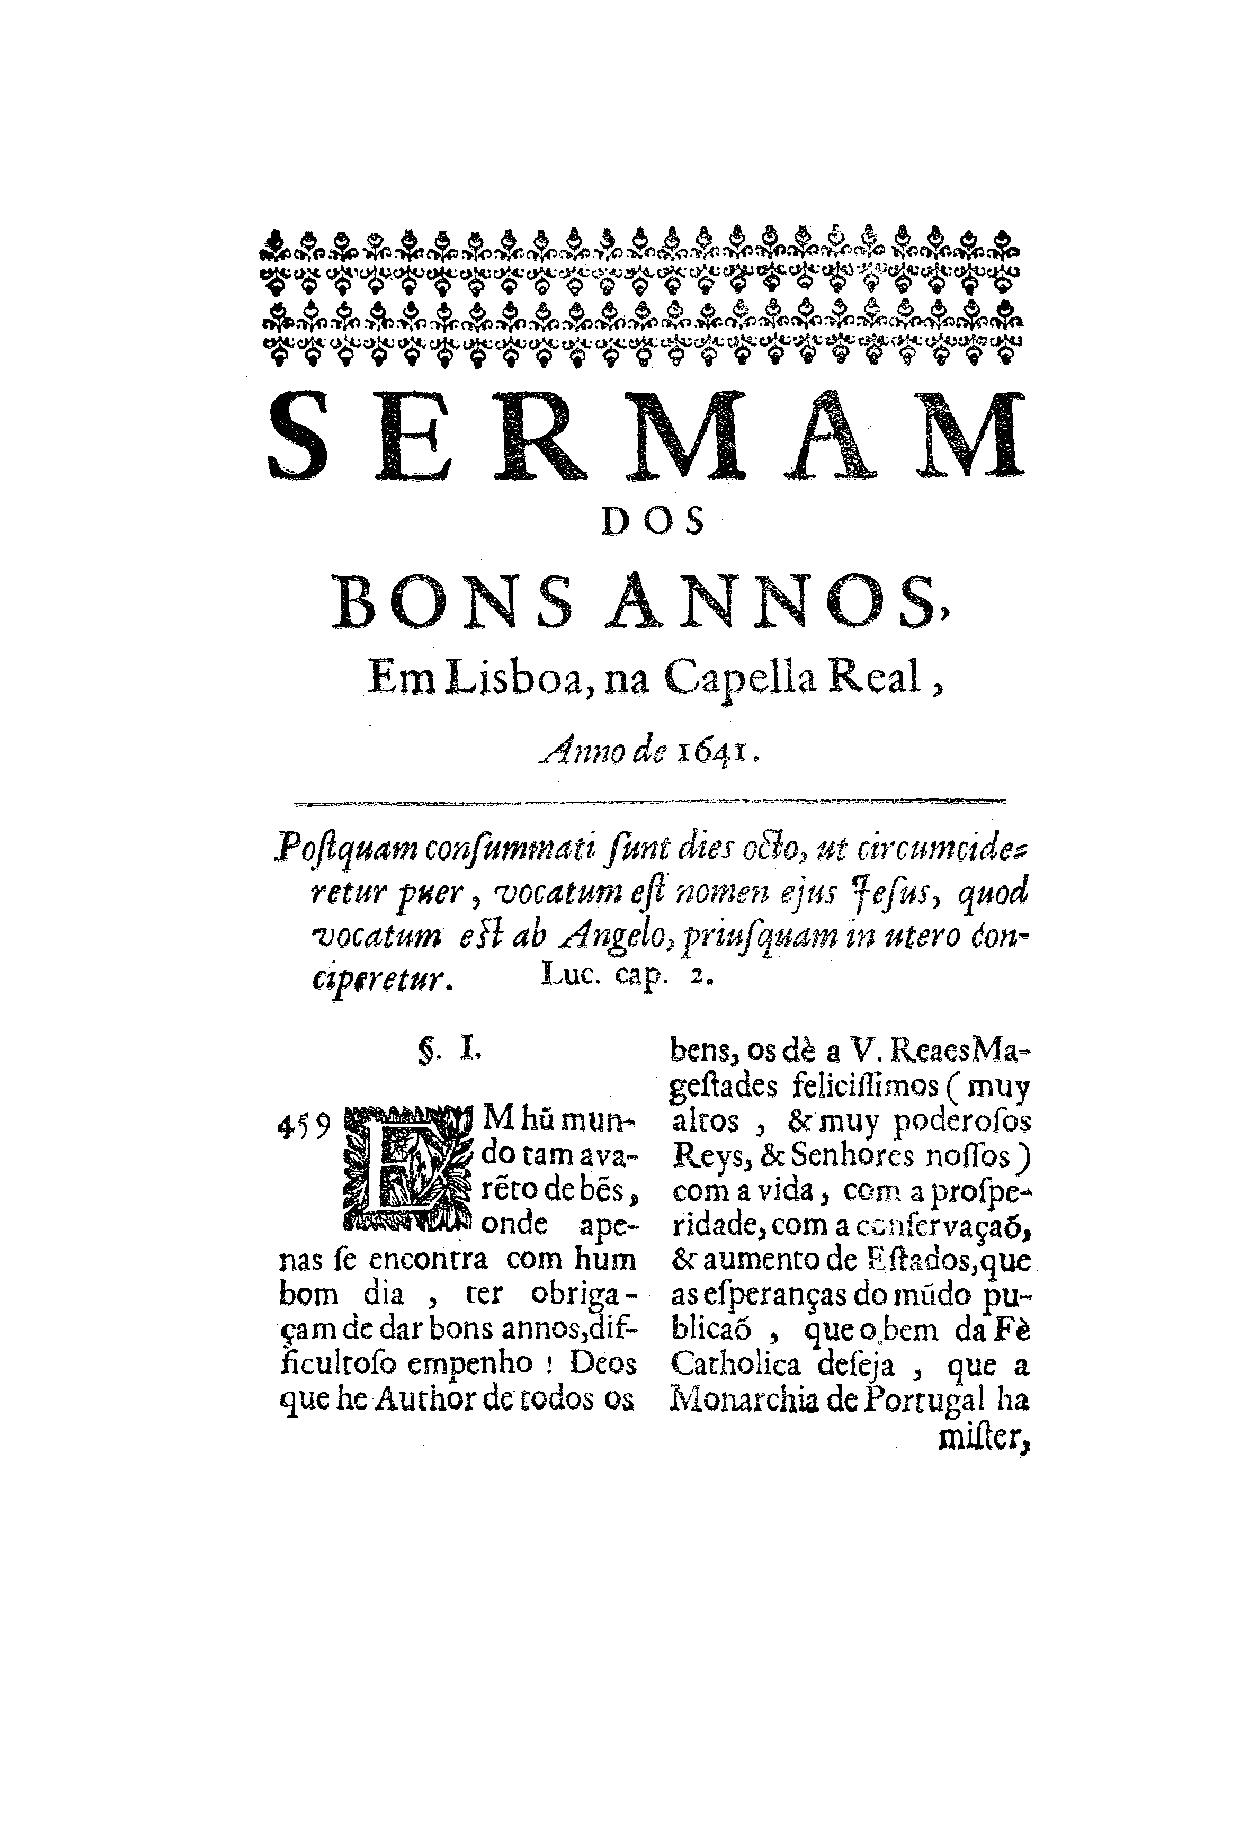
\includegraphics[width=\textwidth]{./imgs/bonsanos.pdf}  
\end{figure}

\pagebreak
\movetoevenpage
\thispagestyle{empty}
\mbox{}\vfill
\noindent{}O sermão postula que a posse do trono português por D.\,João \textsc{iv} estava já profetizada, e assinala o início de um novo tempo de bonança. Em termos mais específicos, adota uma posição ``neosebastianista'', na qual o Rei Encoberto das trovas populares não é D.\,Sebastião, dado efetivamente como morto, mas o novo rei brigantino: o rei ``esperado'' identifica"-se assim com o rei atualmente empossado. O sermão também justifica três medidas tomadas no primeiro ano do governo de D.\,João \textsc{iv}: a restrição de gastos, a premiação de antigos
vassalos e a convivência com os inimigos.

\chapter{Sermão dos Bons Anos}

\begin{quotation}
\noindent{}Em Lisboa, na Capela Real, Ano de 1641
\end{quotation}

\epigraph{\emph{Postquam consummati sunt dies octo, ut circumcideretur puer,
vocatum est nomen ejus Jesus, quod vocatum est ab angelo, priusquam in
utero conciperetur}.}{Lc, 2.}

\section{i}

\noindent{}Em um Mundo tão avarento de bens, onde apenas se encontra com um bom
dia, ter obrigação de dar bons"-anos, dificultoso empenho! Deus, que é
autor de todos os bens, os dê a Vossas Reais Majestades felicíssimos
(mui altos e mui poderosos Reis e Senhores nossos) com a vida, com a
prosperidade, com a conservação e aumento de estados que as esperanças
do Mundo publicam, que o bem da Fé Católica deseja, que a Monarquia de
Portugal há mister e que eu hoje quisera prometer e ainda assegurar.

Em um Mundo, digo, tão avarento de bens, onde apenas se encontra com um
bom"-dia, ter obrigação de dar bons"-anos, dificultoso empenho! E na minha
opinião cresce ainda mais esta dificuldade, porque isto de dar
bons"-anos, entendo"-o de diferente maneira do que comumente se pratica no
Mundo. Os bons"-anos não os dá quem os deseja, senão quem os assegura. A
quantos se desejaram nesta vida, a quantos se deram os bons"-anos, que os
não lograram bons, senão mui infelizes? Segue"-se logo, própria e
rigorosamente falando, que não dá os bons"-anos quem só os deseja, senão
quem os faz seguros. Esta é a dificuldade a que me vejo empenhado hoje,
que o tempo e o Evangelho fazem ainda maior. Em todo o tempo é
dificultoso cousa segurar anos felizes; mas muito mais em tempo de
guerras e em tempo de felicidades. Se o dia dos bens é véspera dos
males; se para merecer uma desgraça, basta ter sido ditoso, quem fará
confiança em glórias presentes, para esperar prosperidades futuras? Se a
campanha é uma mesa de jogo onde se ganha e se perde; se as bandeiras
vitoriosas mais firmes seguem o vento vário que as meneia, quem se
prometerá firmeza na guerra, que derruba muralhas de mármore? E como a
guerra e a felicidade são dois acidentes tão vários; como a Fortuna e
Marte são dois árbitros do Mundo tão inconstantes, como poderei eu
seguramente prometer bons"-anos a Portugal, em tempo que o vejo por uma
parte com as armas nas mãos, por outra com as mãos cheias de felicidade?
Se apelo para o Evangelho, também parece que promete ameaças, mais que
esperanças; porque nos aparece nele um cometa abrasado e sanguinolento,
\emph{ut circumcideretur puer}, e os cometas desta cor sempre foram
fatais aos reinos e formidáveis às monarquias.

\emph{Terret fera regna cometes sanguineum spargens ignem}, disse lá
Sílio. A matéria dos cometas são os vapores, ou exalações da terra
subidas ao céu; e como no mistério da Encarnação subiu ao Céu a terra de
nossa humanidade, que outra cousa parece Cristo hoje com o sangue da
circuncisão, senão um cometa abrasado e sanguinolento, e por isso
funesto e temeroso? Ora com isto se representar assim, com o Evangelho e
o tempo parecer que nos prometem poucas esperanças de felizes anos, do
mesmo tempo e do mesmo Evangelho hei de tirar hoje a prova e segurança
deles Será pois a matéria e empresa do sermão esta: \emph{Felicidades
de Portugal}, juízo dos anos que vêm. Digo dos anos, e não do ano,
porque quem tem obrigação de dar bons"-anos, não satisfaz com um só,
senão com muitos. Funda"-me o pensamento o mesmo Evangelho, que parece o
desfavorecia; porque toda a matéria e sentido dele é um prognóstico de
felicidades futuras.
Toda a matéria do brevíssimo Evangelho que hoje canta a Igreja vem a ser
a circuncisão de Cristo e o nome santíssimo de Jesus. E destes dois
grandes mistérios se compôs uma constelação benigníssima, que tomada no
horizonte oriental de Cristo, foi figura de todo o bem e remédio do
Mundo. que o Senhor havia de obrar em seus maiores anos. S.\,Cirilo:
\emph{Vocatum est nomen ejus !esus, quod interp,etatur Salvator; editus
enim fuit ad toIius mundi salutem, quam sua circumcisione
praefiguravit}. Grande palavra! De sorte que circuncidar"-se Cristo e
chamar"-se Jesus no dia de hoje, foi levantar figura,
\emph{praefiguravit}, aos sucessos dos anos seguintes, à salvação e
felicidades futuras de todo o género humano: \emph{Totius mundi,
salutem, quum sua circumcisione praefiguravit}. Nem desfaz esta verdade
a representação do sanguinolento, com que parece nos atemorizava Cristo
nos efeitos da circuncisão; porque aquele belo infante não é cometa, é
planeta; não é terra subida ao céu, é céu descido à terra. E o céu,
quando se põe de vermelho, que prognostica? O mesmo Cristo o disse,
que não é menos que sua esta matemática: \emph{Serenum erit, rubicundum
est enim caelum}. Quando o céu se veste de vermelho, prognostica
serenidade. Sempre a serenidade foi título natural das púrpuras. E como
aquele Céu animado, como aquele Rei celestial se veste da púrpura de seu
sangue, serenidades e felicidades grandes nos prognostica. que nas ações
do tempo e nas palavras do Evangelho iremos discorrendo por partes.

\section{ii}

\emph{Postquam consummati sunt dies octo, ut circumcideretur puer,
vocatum est nomen ejus Jesus, quod vocatum est ab ungelo, priusquam in
utero conciperetur}.

Comecemos por estas últimas palavras.
Diz S.\,Lucas que, passados os oito dias, termo da circuncisão, lhe
puseram a Cristo por nome Jesus; e nota, antes manda notar o
Evangelista, que este nome foi anunciado pelo Anjo, antes que o Senhor
fosse concebido: \emph{Quod vocatum est ab angelo, priusquam in utero
conciperetur}. Dá razão desta advertência a glossa interlineal, e diz
que foi: \emph{Ne homo videretur machinator hujus nominis}: Para que
não parecesse este glorioso nome maquinado por invento de homens, senão
mandado, como era, pela verdade de Deus. Entrou Cristo no Mundo a
reduzi"-lo com nome de Salvador e Libertador, que isso quer dizer Jesus;
pois para que esta apelidada liberdade não a possa julgar alguém por
invenção e obra humana, seja profetizada e revelada primeiro por um
ministro da Providência Divina: \emph{Quod vocatum est ab angelo,
priusquam in utero conciperetur}.

Não quero referir profecias do bem que gozamos, porque as suponho mui
pregadas neste lugar e mui sabidas de todos; reparar sim, e ponderar o
intento delas quisera. Digo que ordenou Deus que fosse a liberdade de
Portugal, como os venturosos sucessos dela, tanto tempo antes e por tão
repetidos oráculos profetizada, para que, quando víssemos estas
maravilhas humanas, entendêssemos que eram disposições e obras divinas,
e para que nos alumiasse e confirmasse a fé onde a mesma admiração nos
embaraçasse. (Falo de fé menos rigorosa, quanta cabe em matérias não
definidas, posto que de grande certeza.) Alega Cristo um texto do Salmo
\textsc{xl}, em que descreve David o meio extraordinário por onde os
procedimentos injustos de um mau homem dariam princípio à redenção de
todos, como seria traído o Redentor, como o pretenderiam derrubar por
engano do seu estado; e intimando o Senhor o caso aos discípulos, disse
estas particulares palavras: \emph{Dico vobis antequam fiat, ut cum
factum fuerit credatis quia ego sum}. Eu sou este de quem aqui fala David (que assim explicam o lugar Santo Agostinho, Ruperto, Teofilato e outros); e digo"-vos isto antes que aconteça, para que depois de acontecer o creiais.
Notável teologia, por certo! Se o Senhor dissera Digo"-vos estas cousas
para que creiais, antes que aconteçam, facilmente dito estava; isso é fé:
crer o que não se vê; mas dizer as causas antes que se façam, a fim
de que se creiam depois de feitas: \emph{Ut cum factum fueri credatis}?
O que está feito, o que se vê, o que se apalpa necessita de fé?
Algumas vezes sim; porque sucedem casos no Mundo, como este de que
Cristo falava, tão novos e inauditos; sucedem cousas tão raras, tão
prodigiosas e por meios de proporção tão desigual e muitas vezes tão
contrários ao mesmo fim, que, ainda depois de vistas com os olhos, ainda
depois de experimentadas com as mãos, não basta a evidência dos sentidos
para as não duvidar, é necessário recorrer aos motivos da fé para lhes
dar crédito: \emph{Dico vobis antequam fiat, ut cum factum fuerit,
credatis}. Tais considero eu os sucessos nunca imaginados de nosso
Portugal, que, como excessivamente nos acreditam, assim excedem todo o
crédito.
Quis Deus que fossem tantos anos antes e tão vulgarmente profetizados
estes sucessos, não tanto para os esperarmos futuros, quanto para os
crermos presentes; não para nos alentarem a esperança antes de
sucederem, mas para nos confirmaram a fé depois de sucedidos. Haviam de
suceder as cousas de Portugal, como sucederam, de tão prodigiosa
maneira, que, ainda depois de vistas, parece que as duvidamos; ainda
depois de experimentadas, quase as não acabamos de crer: pois
profetize"-se esta venturosa liberdade e ainda o nome felicíssimo do
libertador, muito tempo antes, \emph{priusquam in utero conciperetur},
para que entre as dúvidas dos sentidos, entre os assombros da
admiração, peçam os olhos socorro à fé e creiam o que vêem por
profetizado, quando o não creiam por visto.

Por duas razões se persuadem mal os homens a crer algumas cousas: ou por
muito dificultosas, ou por muito desejadas; o desejo e a dificuldade
fazem as cousas pouco críveis. Era Sara de idade de noventa anos, sobre
estéril; promete"-lhe um anjo que Deus lhe daria fruto de bênção; e diz a
Escritura que se riu e zombou muito disso Sara; e ainda depois de ter um
filho chamou"-lhe Isac, que quer dizer riso: \emph{Risum fecit mihi
Deus}. Estava S.\,Pedro em poder de el"-rei Herodes preso e com apertada
guarda; apareceu"-lhe outro anjo, que lhe quebrou as cadeias e o livrou;
e diz o texto sagrado: \emph{Existimabat autem se visum videre}: que
cuidava Pedro que aquilo era sonho e ilusão. Pois Pedro, pois Sara,
que incredulidade é esta? Vê"-se Sara com um filho nos braços, e
chama"-lhe riso? Vê"-se Pedro com as cadeias fora das mãos, e chama"-lhe
sonho? Assim havia de ser, porque ambas eram cousas muito
dificultosas e ambas muito desejadas. Desejava Sara um filho, como a
sucessão de sua casa; desejava Pedro a liberdade, como a mesma liberdade
bem da Igreja. A sucessão de Sara estava em poder de noventa anos; a
liberdade de Pedro estava em poder de Herodes e de seus soldados; e como
a dificuldade era tão grande e o desejo igual à dificuldade, ainda que
viam com seus alhos e tinham nas mãos o que desejavam, a Sara,
parecia"-lhe cousa de riso, a Pedro parecia"-lhe cousa de sonho. Que Sara
estéril haja de ter filho! Que a prosápia real portuguesa esterilizada e
atenuada na décima sexta geração, haja de ter descendente que lhe
suceda! Que Sara, depois de noventa anos! que a coroa de Portugal
depois de sessenta! O que não teve quando estava na flor de sua idade, o que não
teve quando estava com todas as suas forças o viesse alcançar depois de
tão envelhecida e quebrantada? Muito desejávamos, muito suspirávamos por
este bem, mas quanto maior era o desejo, tanto mais parecia. e quase parece ainda
cousa de riso: \emph{Risum fecit mihi Deus}. Que Pedro em poder de
el"-rei Herodes; que Portugal em poder não de um. senão de muitos reis
que o dominavam, lhes houvesse de escapar das mãos tão facilmente! Que
Pedro cercado de guardas: \emph{Quator quaternionibus militum}; que
Portugal, presidiado de infantaria em tantos castelos, em tantas
fortalezas, sem se arrancar uma espada, sem se disparar um arcabuz;
conseguisse em uma hora sua liberdade! Era empresa esta tão dificultosa,
representava"-se tão impossível ao discurso humano, que ainda agora
parece que é sonho e ilusão: \emph{Existimabat se visum videre}. Assim
lhes aconteceu aos filhos de Israel, quando se viram livres do cativeiro
de Babilónia: \emph{In convertendo Dominus captivitatem Sion facti
sumus} (lê o hebreu) \emph{sicut somniantes}: que incrédulos, de
admirados, tinham a verdade por imaginação e cuidavam que estavam
sonhando o que viam com os olhos abertos. E como os sucessos de nossa
restauração eram matérias de tão dificultoso crédito, que, ainda depois
de vistos, parecem sonho e quase se não acabam de crer, ordenou Deus que
fossem tanto tempo antes, como tão singulares circunstâncias e com o
nome do mesmo libertador profetizadas, para que a certeza das profecias
desfizesse os escrúpulos da experiência; para que, sendo objecto da fé,
não parecesse ilusão dos sentidos; para que, revelando"-as tantos
ministros de Deus, se visse que não eram inventos dos homens: \emph{Ne
homo videretur machinator hujus nominis, quod vocatum est ab angelo,
priusquum in utero conciperetur}.

\section{iii}

Temos considerado o \emph{priusquam}, vamos agora ao \emph{postquam:
Postquam consummati sunt dies octo, ut circumcideretur puer}. O que aqui
pondera e sente muito a piedade dos santos, principalmente S.\,Bernardo,
é que, nascido de oito dias, sujeitasse o Senhor aquele corpozinho tenro
ao duro golpe da circuncisão. Tão depressa? Aos oito dias já derramando
sangue? Desta pressa se espantam os Doutores; mas eu não me espanto
senão deste vagar. Que venha Cristo a remir, e que espere dias? E que
espere horas? E que espere instantes? Quem cuida que é pouco tempo
oito dias, mal sabe o que é esperar pela Redenção.
Quando Cristo se encontrou com os discípulos de Emaús, iam eles contando
a história de seu Mestre e a causa que os levava peregrinos por esse
Mundo, e disseram estas notáveis palavras: \emph{Nos autem sperabamus,
quia ipse esset redempturus Israel; et nunc super haec omnia tertia dies
est hodie}: Nós esperávamos que este nosso Mestre havia de remir o povo
de Israel; e no cabo de tudo isto, vemos agora que já se vão passando
três dias. Três dias? Pois que muito é isso? Que espaço de tempo são
três dias para uns homens desmaiarem? Para uns homens se entristecerem?
Para uns homens se desesperarem tanto? Não se desesperavam, porque
eram três dias, senão porque eram três dias de esperar pela Redenção.
Esperavam aqueles discípulos que o Senhor havia de remir a Israel:
\emph{Nos autem sperabamus quia ipse esset redempturus Israel}. E para
quem está cativo, para quem espera pela Redenção, três dias é muito
tempo: \emph{Et nunc super haec omnia}: como se foram passadas três
eternidades: \emph{Tertia dies est hodie}: Já se vão passando três dias;
é muito tempo para quem espera pela Redenção, quanto mais tempo seriam
os oito dias que se dilatou a circuncisão de Cristo, pois
esperava o Mundo neles, que começasse o Senhor a derramar o sangue e dar
o preço com que o remiu!
Não há dúvida que foi muito cedo para a dor, mas não foi muito cedo para
o remédio; foram poucos dias para quem vivia. mas muitos para quem
esperava. Bem o entendeu assim o Evangelista; porque, havendo de contar
estes oito dias, veja"-se
o aparato de palavras com que o faz: \emph{Postquam consummati sunt};
depois que foram consumados: parece que armava a dizer oito séculos,
ou oito mil anos, segundo a grandeza vagarosa e a ponderação das
palavras; e no cabo disse: \emph{dies octo}, oito dias; que, como eram
dias de esperar Redenção, ainda Que não foram mais que oito, pareciam
uma duração muito comprida, e que não acabavam de chegar, segundo
tardavam: \emph{Postquam consummati sunt}.

E se oito dias de esperar pela redenção, e ainda três dias, é tanto
tempo; quanto seria, ou quanto pareceria, não três dias, nem oito dias,
não três anos, nem oito anos, senão sessenta anos inteiros nos quais
Portugal esteve esperando sua redenção, debaixo de um cativeiro tão duro
e tão injusto! Não me paro a o ponderar; porque em dia tão de festa, não
dizem bem memórias de tristezas, ainda que os males passados, parte vêm
a ser de alegria. O que digo é que nos devemos alegrar com todo o
coração e dar imortais graças a Deus, pois vemos tão felizmente logradas
nossas esperanças. Nem nos pese de ter esperado tão longamente; porque
se há de recompensar a dilação da esperança com a perpetuidade da posse.
Perguntam os Teólogos como São Tomás na terceira parte, porque se
dilatou tanto tempo o mistério da Encarnação, porque não desceu o Verbo
Eterno a remir o Mundo, senão depois de tantos anos? Várias razões dão
os Doutores: a de Santo Agostinho é muito própria do que queremos dizer:
\emph{Diu fuit expectandus, semper tenendus}. Quis o Verbo Eterno que
esperassem os homens e suspirassem tantos séculos por sua vinda, porque
era bem que fosse muito tempo esperado um bem que havia de ser sempre
possuído. Haviam os homens de gozar para sempre a presença de Cristo,
havia o Verbo de ser homem perpetuamente: porque, \emph{Quod semel
assumpsit nunquam demisit}, o que uma vez tomou, nunca mais o largou;
seja pois este bem por muito tempo esperado, pois há de ser por todo o
tempo possuído, e mereça com as dilações da esperança a perpetuidade da
posse: \emph{Diu fuit expectandus, semper tenendus}.
Não necessita de acomodação o lugar; de firmeza sim, pelas dependências
que tem no futuro; mas um espírito profético e português nos fiará a
conjectura desta tão gostosa verdade. S.\,Frei Gil, religioso da sagrada
ordem de S.\,Domingos, naquelas suas tão celebradas profecias, diz desta
maneira: \emph{Lusitania sanguine orbata regio diu ingemiscet}: A
Lusitânia o reino de Portugal, morrendo seu último rei sem filho
herdeiro, gemerá e suspirará por muito tempo; \emph{Sed propitius tibi
Deus}: Mas lembrar"-se"-á Deus de vós, ó Pátria minha, diz o Santo; \emph{Et
insperate ab insperato redimeris}: E sereis remida não esperadamente
por um rei não esperado. E depois de assim remido, depois de assim
libertado Portugal, que lhe sucederá? \emph{Africa debellabitur}:
Será vencida e conquistada África. \emph{Imperium ottomanum ruet}: O
império otomano cairá sujeito e rendido a seus pés. \emph{Domus Dei
recuperabitur}: A casa santa de Jerusalém será finalmente recuperada. E
por coroa de tão gloriosas vitórias, \emph{Aetas aurea reviviscet}.
Ressuscitará a idade dourada. \emph{Pax ubique erit}.
Haverá paz universal no Mundo. \emph{Felices qui viderint}: Ditosos e
bem"-aventurados os que isto virem.
Até aqui S.\,Frei Gil profetizando. De sorte que, assim como antes da
Redenção houve suspirar e gemer, assim depois da Redenção haverá possuir
e gozar; e assim como os suspiros e gemidos duraram por tantos anos,
assim as
felicidades e bens permanecerão sem termo e sem limite. O muito, quer
Deus que não custe pouco, e era justo que a tanta glória precedesse
tanta esperança, e que quem havia de gozar sempre, suspirasse muito:
\emph{Lusitania diu ingemiscet. Diu fuit expectandus, semper tenendus}.

E já que vai de esperanças, não deixemos passar sem ponderação aquelas
palavras misteriosas da profecia: \emph{Insperate ab insperato
redimeris}. De propósito reparei nelas, para refutar com suas próprias
armas alguma relíquia, que dizem que ainda há daquela seita ou
desesperação dos que esperavam por el"-rei D.\,Sebastião, de gloriosa e
lamentável memória. Diz a profecia: \emph{Insperate ab insperato
redimeris}. Que seria remido Portugal não esperadamente por um rei não esperado.
Segue"-se logo, evidentemente, que não podia el"-rei D.\,Sebastião ser o
libertador de Portugal, porque o libertador prometido havia de ser um
rei não esperado: \emph{Insperate ab insperato}; e el"-rei D.\,Sebastião
era tão esperado vulgarmente, como sabemos todos. Assim que os mesmos
sequazes desta Opinião, com seu esperar, destruíram sua esperança;
porque quanto o faziam mais esperado, tanto confirmavam mais que não era
ele o prometido; podendo"-se"-lhe aplicar propriamente aquelas palavras
que S.\,Paulo disse de Abraão: \emph{Contra spem in spem credidit}: que
creram em uma esperança contrária à sua mesma esperança; porque pelo mesmo que
esperavam, tinham obrigação de não esperar.

Mas ainda que concedamos que os Portugueses não souberam esperar, não
lhes neguemos que souberam amar, e com muita ventura; que talvez
buscando a um rei morto, se vêm a encontrar com um vivo. Morto buscava a
Madalena a Cristo na sepultura, e a perseverança e amor com que insistiu
em o buscar morto, foi causa de que o Senhor lhe enxugasse as lágrimas e
se lhe mostrasse vivo. Grande exemplar temos entre mãos! Assim como a
Madalena, cega de amor, chorava às portas da sepultura de Cristo, assim
Portugal, sempre amante de seus reis, insistia ao sepulcro de el"-rei D.\,Sebastião, chorando e suspirando por ele; e assim como a Madalena no
mesmo tempo tinha a Cristo presente e vivo, e o via com seus olhos e lhe
falava e não o conhecia, porque estava encoberto e disfarçado, assim
Portugal tinha presente e vivo a el"-rei nosso senhor, e o via e lhe
falava e não conhecia. Porquê? Não só porque estava, senão porque ele
era o encoberto. Ser o encoberto e estar presente, bem mostrou Cristo
neste passo que não era impossível. E quando se descobriu Cristo? Quando
se manifestou este Senhor encoberto? Até esta circunstância não faltou
no texto. Disse a Madalena a Cristo: \emph{Tulerunt Dominum meum}:
Levaram"-me o meu Senhor; e o Senhor não lhe deferiu. \emph{Nescio ubi
posuerunt eum}: queixou"-se que não sabia onde lho puseram; e dissimulou
Cristo da mesma maneira. \emph{Si tu sustulisti eum}: Se vós, Senhor, o
levastes, \emph{dicito mihi}, dizei"-mo; e ainda aqui se deixou o Senhor
estar encoberto sem se manifestar. Finalmente, alentando"-se a Madalena
mais do que sua fraqueza permitia, e tirando forças do mesmo amor,
acrescentou: \emph{Et ego eum tollam}: E eu o levantarei; e tanto
que disse, eu o levantarei: \emph{Ego eum tollam}: então se descobriu
o Senhor, mostrando que ele era por quem chorava; e a Madalena o
reconheceu e se lançou a seus pés.
Nem mais nem menos Portugal, depois da morte de seu último rei.
Buscava"-o por esse Mundo, perguntava por ele, não sabia onde estava,
chorava, suspirava, gemia, e o rei vivo e verdadeiro deixava"-se estar
encoberto e não se manifestava,
porque não era ainda chegada a ocasião; porém tanto que o Reino, animoso
sobre suas forças, se deliberou a dizer resolutamente: \emph{Ego eum
tollam}: eu o levantarei e sustentarei com meus braços, então se
descobriu o encoberto Senhor, porque então era chegado o tempo,
dizendo"-nos aos Portugueses o que diz S.\,Gregório que disse Cristo à
Madalena manifestando"-se: \emph{Recognosce eum, a quo recognosceris}:
Reconhecei a quem vos reconhece; reconhecei por rei, a quem vos
reconhece por vassalo. Então sim, e não antes; então sim, e não depois;
porque aquele e não outro era o tempo oportuno e determinado de dar
princípio à nossa redenção.

Recebeu Cristo o golpe da circuncisão e deu princípio à Redenção do
Mundo, não antes nem depois, senão pontualmente aos oito dias:
\emph{Dies octo, ut circumcideretur puer}. Pois porque antes, ou porque
não depois? Não se circuncidara ao dia sétimo? Não se circuncidara ao
dia nono? Porque não antes nem depois, senão ao oitavo? A razão foi
porque as cousas que faz Deus e as que se hão de fazer bem feitas, não
se fazem antes, nem depois, senão a seu tempo. O tempo assinalado nas
Escrituras para a circuncisão era o dia oitavo, como se lê no
\emph{Gênesis} e no \emph{Levítico}: \emph{Die octavo circumcideretur
infantulus}. E por isso se circuncidou Cristo, sem se antecipar, nem
dilatar aos oito dias: \emph{Postquam consummati sunt dies octo}; porque
como o Senhor remiu o gênero humano por obediência aos decretos divinos,
o tempo que estava assinalado na lei para a circuncisão era o que estava
predestinado para dar princípio à redenção do Mundo. Da mesma maneira se
deu princípio à redenção e restauração de Portugal em tais dias e em tal
ano, no celebradíssimo de 40, porque esse era o tempo oportuno e
decretado por Deus; e não antes nem depois, como os homens quiseram.
Quiseram os homens que fosse antes, quando sucedeu o levantamento de
Évora; quiseram os homens que fosse depois, quando assentaram que o dia
da aclamação fosse o 1º de Janeiro, hoje faz um ano; mas a Providência
Divina ordenou se antecipasse, para que pontualmente se desse princípio
à restauração de Portugal a seu tempo: \emph{Postquam consummati sunt
dies octo}.

\section{v}

Daqui fica tacitamente respondida uma não mal fundada admiração, com que
parece podíamos reparar os Portugueses, em que os sereníssimos duques de
Bragança vivessem retirados todos estes anos, sem acudirem à liberdade
do Reino, como legítimos herdeiros que eram dele. Respondido está;
declaro mais a resposta: Cristo, Redentor nosso, ainda em quanto homem,
como provam muitos Doutores, era legítimo herdeiro da coroa de Israel:
\emph{Dabit illi Dominus Deus sedem David Patris ejus: et regnabit}.
Tinha tiranizado este reino Herodes, homem estrangeiro, a quem por este
e por muitos outros títulos não pertencia; e como, sobre ter usurpado o
Reino, lhe quisesse tirar a vida a Cristo, diz o texto, que o Senhor se
lhe não opôs, antes se retirou para o Egipto: \emph{Secessit in
Aegyptum}. Notável ação! Não sois vós, Senhor, o verdadeiro Rei de
Israel, como legítimo herdeiro seu, que, ainda que não empunhais o
ceptro, Rei sois e Rei nascestes, e assim o confessam as nações e reis
estrangeiros: \emph{Ubi est qui natus est Rex Judiorum}? Pois como vos
retirais agora, como vos não apondes à tirania de Herodes, como ides
viver ao Egipto, e tantos anos? Não vedes o que padecem tantos
inocentes? Não ouvis que já chegam ao Céu as vozes da lastimada Raquel,
que chora seus filhos: \emph{Vox in Rama audita est, ploratus et
ululatus multus, Raquel plorans filios suos?} Pois se a vós, como a Rei
natural, incumbe a restauração do Reino, como vos retirais da empresa?
Nem me aleguem em contrário os poucos dias que tinha o Senhor de vida ou de
idade, depois dos oito da circuncisão, porque na mesma circuncisão e na
mesma retirada do Egito tinha e lhe sobejava tudo o que era necessário
para livrar do cativeiro os que nele tinham a esperança da liberdade. Ou
Cristo os havia de remir com o sangue próprio, ou com o alheio: se com o
próprio, bastava uma só gota do sangue da circuncisão, para remir não só
o reino de Israel, senão todo o Mundo. Se com o sangue alheio o mesmo
anjo que disse a S.\,José: \emph{Fuge in Aegyptum}, podia fazer a Herodes
e a todos seus presídios e soldados, o que outro anjo fez aos exércitos
de el"-rei Senaquerib, matando em uma noite oitenta e cinco mil dos que
sitiavam a mesma Jerusalém. Pois se isto era não só possível, mas fácil,
ao legítimo e verdadeiro Rei de Israel, porque o não executou então?
Porque não era ainda chegado o tempo, diz excelentemente S.\,Pedro
Crisólogo: \emph{Cedens tempori non Herodi}. Tinha decretado e disposto,
que o tempo da Redenção fosse dali a trinta e três anos e se a
Providência Divina, que tudo pode, espera pelas disposições e
circunstâncias do tempo; quanto mais a providência humana, a qual o não
seria, se com toda a atenção e vigilância as não observasse, aguardando
pelas mais convenientes e oportunas que Deus e o mesmo tempo lhe
oferecesse! Assim que, podiam responder aqueles príncipes, como
legítimos e naturais senhorios e herdeiros da coroa de seus avós, o que
em semelhante caso disseram os famosos Macabeus, assim antes como depois
de restituídos ao seu próprio patrimônio: \emph{Neque alienam terram
sumpsimus, negue aliena detinemus, sed haereditatem patrum nostrorum,
quae injuste ab aliquo tempore ab inimicis nostris possessu est; nos
vero tempus habentes vindicamus haereditatem patrum nostrorum}.

E foi de tanta importância esperar pela oportunidade do tempo, que por
esta dilação se veio a lograr aquela primeira máxima de toda a razão de
estado, assim da Providência Divina, como da providência humana, que é
saber concordar estes dois extremos: conseguir o intento e evitar o
perigo. Já perguntamos que razão teve Cristo para receber a circuncisão
ao oitavo dia conforme a Lei. Agora pergunto: que razão teve a Lei para
mandar que a circuncisão se fizesse ao oitavo dia? A circuncisão naquele
tempo era o remédio do pecado original, como hoje o é o batismo, bem que
com diferente perfeição. Pois se na circuncisão consistia o remédio do
pecado original, e a liberdade das almas cativas pelo pecado; porque não
mandava Deus que se circuncidassem os meninos logo quando nasciam, ou ao
terceiro ou ao quarto dia, senão ao oitavo? A razão literal foi, diz
o Abulense, porque quis Deus aplicar o remédio de tal maneira, que se
evitasse o perigo: \emph{Quia ante octo dies potest esse vitae
periculum}. Quando os meninos nascem, cm todos aqueles primeiros sete
dias correm grande perigo de vida, porque são dias críticos e
arriscados, como dizem Aristóteles e Galeno; pois ainda que o remédio
dos recém"-nascidos e sua espiritual liberdade consistia na circuncisão,
não se circuncidem, diz a Lei, senão ao oitavo dia, passados os sete que
essa é a excelente razão de estado da providência de Deus saber dilatar
o remédio, para escusar o perigo: dilate"-se o remédio da circuncisão até
o oitavo dia, para que se evite o perigo da vida, que há do primeiro ao
sétimo: \emph{Quia ante octo dies potest esse vitae periculum}.

Se Portugal se levantara enquanto Castela estava vitoriosa, ou, quando
menos, enquanto estava pacífica, segundo o miserável estado em que nos
tinham posto, era a empresa mui arriscada. eram os dias críticos e
perigosos; mas como a Providência Divina cuidava tão particularmente de
nosso bem, por isso ordenou que se dilatasse nossa restauração tanto
tempo, e que se esperasse a ocasião oportuna do ano de quarenta, em que
Castela estava tão embaraçada com inimigos, tão apertada com guerras de
dentro e de fora; para que, na diversão de suas
impossibilidades, se lograsse mais segura a nossa resolução. Dilatou"-se
o remédio, mas segurou"-se o perigo. Quando os Filisteus se quiseram
levantar contra Sansão, aguardaram a que Dalila lhe tivesse presas e
atadas as mãos, e então deram sobre ele. Assim o fizeram os Portugueses
bem advertidos. Aguardaram a que Catalunha atasse as mãos ao Sansão que
os oprimia, e como o tiveram assim embaraçado e preso. então se
levantaram contra ele tão oportuna como venturosamente.
Mas vejo que me dizem os lidos na Escritura, que é verdade que os
Filisteus se levantaram contra Sansão, mas que ele soltou as ataduras.
voltou sobre eles e desbaratou"-os a todos. Primeiramente muito vai de
Sansão a Sansão e de Filisteus a Filisteus. Mas dado que em tudo fora a
semelhança igual, esta mesma réplica confirma mais o meu intento. Não
tiveram bom sucesso os Filisteus, porque ainda que nós os imitamos em
parte, eles não nos deram exemplo em tudo. Intentaram, mas não
conseguiram; porque as diligências que fizeram não as aplicaram a tempo.
As diligências que fizeram os Filisteus contra Sansão, foi atarem"-lhe as
mãos e cortarem"-lhe os cabelos; mas não aproveitaram estes efeitos,
ainda que se obraram: porque, devendo"-se fazer ao mesmo tempo,
fizeram"-se em diversos. Quando lhe ataram as mãos, deixaram"-lhe ficar os
cabelos. com que teve força para se desatar; quando lhe cortaram os
cabelos deixaram"-lhos crescer outra vez com que teve mãos para se
vingar. Pois que remédio tinham os Filisteus para se livrarem de todo e
acabarem de uma vez com Sansão? O remédio era fazerem como nós
fizemos e como nós fazemos e como nós havemos de fazer: enquanto Sansão
está com as mãos atadas, cortar"-lhe os cabelos no mesmo tempo, e
acabou"-se Sansão. Assim o podiam vencer os Filisteus com muita
facilidade, que doutra maneira não seria tão fácil. Porque se lhe não
cortassem os cabelos, teria forças para desatar as mãos, e se desatassem
as mãos, seria necessária muita força para lhe cortar os cabelos. Tanto
como isto importa executar os remédios a tempo, como nós, por mercê de
Deus, o temos feito até agora tão felizmente, conseguindo a maior
empresa e evitando o menor perigo; porque soubemos esperar pelos dias
oportunos, como mandava a Lei esperar pelos da circuncisão: \emph{Dies
octo, ut circumcideretur puer.}

\section{vi}

\emph{Ut circumcideretur puer vocatum est nomen ejus Jesus}. Tanto que
se circuncidou o Menino, logo se chamou Salvador. Mas com que
consequência? pergunta S.\,Bernardo: \emph{Circumciditur puer et
vocatur Jesus; quid sibi vult ista connexio?} Que parentesco tem o nome
com a ação? Que combinação tem o salvar com o circuncidar"-se? Três
razões acho nos santos; duas repito, uma só pondero. S.\,Bernardo e
Eusébio Emisseno, dizem que foi a circuncisão de Cristo: \emph{Totius
superfluitatis abjectio}: Uma estreita e mui reformada privação de todo
o supérfluo. Vinha Cristo como Rei e Redentor do Mundo a remi"-lo e
restaurá"-lo, e a primeira cousa que fez, como a mais necessária e
importante, foi estreitar"-se em sua Pessoa, cercear demasias, cortar
superfluidades e fazer uma pragmática geral com seu exemplo:
\emph{Totius superfluitatis abjectio}. Muitas graças sejam dadas a Deus,
que para confirmação ou imitação desta grande razão de estado divina,
não temos necessidade de cansar a memória, senão de abrir os olhos; não
de resolver escrituras antigas, senão de venerar e amar exemplos
presentes. Assim obra quem assim reina; assim sabe libertar quem assim
sabe estreitar: \emph{Ut circumcideretur puer, vocatum est nomen ejus
Jesus}.

A segunda razão é de Santo Epifânio, e diz que foi: \emph{Ut confirmaret
circumcisionem, quam olim instituerat ejus adventui servientem}: Que
quis o Redentor confirmar desta maneira e honrar a circuncisão, pelo que
antes da sua vinda tinha servido. Bem advertido, mas muito melhor
imitado. Parece que os decretos do Governo de Portugal e os decretos da
Providência Divina correram parelhas (quanto pode ser) na sua e na nossa
redenção. Decretou Deus que à circuncisão se lhe confirmassem suas
antigas honras. havendo respeito ao bem que tinha servido: e o mesmo
decreto se passou cá, e com muita razão: \emph{Ut confirmaret
circumcisionem ejus adventui servientem}. Tinha servido a circuncisão no
tempo passado e na Lei Velha, pois honre"-se no tempo presente e
premeie"-se na Lei Nova; que não é bem que a felicidade geral venha a
ser infortúnio dos que serviram. Que a circuncisão, que tinha tantos
anos de serviços, que a circuncisão, que tinha derramado tanto sangue,
houvesse de ser desgraçada, porque o mundo foi venturoso, não estava
isso posto em razão. Pois baixe um decreto que lhe confirme
efectivamente todas as honras passadas: \emph{Ut confirmaret
circumcisionem, quam olim instituerat}; que é bem que a Lei da Graça
premeie não só os serviços seus, senão os da Lei Antiga, para mostrar,
nisso mesmo, que é Lei da Graça.
Oh! que grande política esta, assim humana, como divina! El"-rei Assuero
mandava ler as histórias e crônicas do reino, para fazer mercês aos que
em tempo de seus antecessores tinham servido. El"-rei Salomão sustentava
de sua própria mesa aos filhos de Berzelai, por serviços feitos em tempo
e à pessoa de David; e ó Rei dos reis, Cristo Redentor nosso, quando no
Monte Tabor desembargou suas glórias (que também pode ser expediente
estarem embargadas por algum tempo), repartiu"-as a três que serviam e a
dois que tinham servido; a S.\,Pedro, a S.\,João e a Santiago, porque
atualmente serviam; e a Moisés e a Elias, um vivo e outro defunto,
porque tinham servido em tempos passados. Assim recebe Cristo e autoriza
hoje a circuncisão, conforme as honras do tempo antigo, não porque se
quisesse servir dela, que já estava muito envelhecida e a queria
aposentar, senão pelo bem que dantes tinha servido: \emph{Ejus odventui
servientem}.

A terceira e última razão é de Santo Ambrósio, de Santo Agostinho, de S.\,João Crisóstomo, de Santo Tomás e ainda de S.\,Paulo, ou quando menos
fundada em sua doutrina, e é esta (alego tantos Doutores pela
dificuldade da razão): \emph{Ea ratione pro nobis circumcisus est, ut
circumcisionem auferret}: Recebeu Cristo a circuncisão, porque, como
autor da Lei Nova, queria tirar do Mundo a circuncisão. Estranha
sentença! Pois porque Cristo queria tirar do Mundo a circuncisão, por
isso recebe e executa em si a mesma circuncisão? Antes parece que para
a tirar do Mundo havia de entrar condenando"-a, desterrando"-a,
proibindo"-a sob graves penas, e não a admitindo por nenhum caso.
Pouco sabe das razões verdadeiras de estado quem assim discorre.
Circuncida"-se Cristo para tirar do Mundo a circuncisão, porque quem
entra a
introduzir uma lei nova, não pode tirar de repente os abusos da velha.
Há de permitir com dissimulação para tirar com suavidade; há de deixar
crescer o trigo com cizânia, para arrancar a cizânia. quando não faça
mal às raízes do trigo. Todo o zelo é mal sofrido, mas o zelo português
mais impaciente que todos. A qualquer relíquia dos males passados, a
qualquer sombra das desigualdades antigas, já tomamos o céu com as mãos,
porque não está tudo mudado, porque não está emendado tudo. Assim se
muda um reino? Assim se emenda uma monarquia? Tantos entendimentos assim
se endireitam? Tantas vontades tão diferentes assim se temperam? Rei era
Cristo, e Rei Redentor, e nenhuma cousa trazia mais diante dos olhos,
que extinguir os usos da Lei Velha e renovar e introduzir os preceitos
da Nova; e com ter
sabedoria infinita e braços onipotentes, ao cabo de trinta e três anos
de reino, muitas cousas deixou como as achara, para que seu sucessor S.\,Pedro as emendasse. Já Cristo não estava vivo, quando se rasgou o véu do
templo, figura da Lei Antiga. E que cousa se podia representar mais
fácil, que romper um tafetá em trinta e três anos? Pouco e pouco se
fazem as cousas grandes, e não há melhor arbítrio para as concluir com
brevidade, que não as querer acabar de repente.
Instituiu Cristo, Redentor nosso, o sacramento da Eucaristia, e
instituiu"-o na mesma mesa em que estava o cordeiro legal. Pois, Senhor
meu, que combinação é esta, ou que companhia? O cordeiro com o
sacramento? As cerimônias da Lei Velha com os mistérios da Nova na mesma
mesa? Sim, que assim era necessário que fosse, para que viesse a ser
o que era necessário. Queria Cristo introduzir o sacramento e lançar
fora o cordeiro da Lei. e para isso permitiu que o cordeiro estivesse
embora na mesma mesa com o sacramento, que desta maneira se desterram
com suavidade as sombras das leis velhas, e se vão introduzindo e
conciliando os resplendores das novas. Estejam agora juntos o sacramento
e o cordeiro, que amanhã irá fora o cordeiro, e ficará o sacramento. Com
este vagar faz Deus as cousas, e assim quer que as façam os que estão em
seu lugar (quando elas o sofrem); e tenha mais paciência o zelo, não
seja tão estreito de coração. Mais dói aos reis que aos vassalos
dissimular com algumas cousas; mas por força se hão de fazer assim, para
se não fazerem por força. Muito lhe doeu a Cristo, gotas de sangue lhe
custou contemporizar com a circuncisão; mas foi necessário dissimular
com dor, para remediar mm sucesso. Não é o mesmo permitir que aprovar,
antes o que se permite já se supõe condenado. A benevolência e
dissimulação, como são afetos da mesma cor, equivocam"-se facilmente nas
aparências; e quantas vezes se choraram ruínas, os que se invejaram
favores! Vem a ser indústria no príncipe, o que é razão de estado no
lavrador, que as espigas que há de cortar, essas abraça primeiro. Assim
abraçou Cristo a circuncisão, porque a queria cortar e arrancar do
Mundo: \emph{Ea ratione circumcisus est, ut circumcisionem auferret},
mostrando na suavidade desta razão, e nas outras cousas por que se
circuncidou, quão bem se proporcionava com os meios o nome que lhe
puseram de Salvador: \emph{Ut circumcideretur puer, vocatum est nomen
ejus Jesus}.

Mas porque se chamou Salvador? Porque não tomou outro nome? Que o não
tomasse de algum atributo de sua divindade, bem está, pois vinha a ser
homem! mas ainda em quanto homem tinha Cristo a maior dignidade da
terra, que era a de rei. Pois já que havia de tomar o nome do ofício e
não da pessoa, porque não se chamou Rei, porque se chamou Salvador? A
razão deu"-a Tertuliano: \emph{Gratius illi erat pietatis nomen, quam
majestatis}: Deixou Cristo o nome de rei e tomou o de Salvador, porque
estimava mais o nome de piedade, que o título de majestade. O nome de
Rei era nome majestoso, o nome de Salvador era nome piedoso; o nome de
Rei dizia imperar, o nome de Salvador dizia libertar; e fazendo o Senhor
a eleição pela estimação, tomou o de nosso remédio, deixou o de sua
grandeza. Por isso os anjos, na embaixada que deram aos pastores,
puseram primeiro o nome de Salvador e depois o de Ungido: \emph{Quia
natus est vobis hodie Salvator, qui est Christus Dominus}. E por isso no
título da cruz se chamou o Senhor Jesus Rei. e não Rei Jesus:
\emph{Jesus Nazarenus, Rex Judaeorum}; para mostrar no princípio e no
fim da vida, que estimava mais o exercício de nossa liberdade, que a
grandeza de sua majestade: \emph{Gratius illi erat pietatis nomen, quam
majestatis}.
Se os corações puderam discorrer sensivelmente, quanto melhor falaram
neste passo, do que os poderá copiar a língua? Isto que Tertuliano disse
pelo primeiro Libertador do gênero humano, pudéramos nós dizer com ação
de graças
pelo segundo libertador de Portugal, o qual nesta felicíssima e
verdadeiramente real arção mostrou bem quanto mais estimava o nome da
piedade, que o título da majestade; pois convidado tantas vezes para a
grandeza, rejeitou generosamente o ceptro; e agora chamado para o
remédio, aceitou animosamente a coroa: \emph{Gratius illi erat pietatis
nomen, quam majestatis}. Rei não por ambição de reinar, senão por
compaixão de libertar; rei verdadeiramente imitador do Rei dos reis, que
sobre todos os títulos de sua grandeza estimou o nome de Libertador e
Salvador: \emph{Vocatum est nomen ejus Jesus}.

\section{vii}

Acabou"-se o Evangelho, e eu tenho acabado o sermão. Mas vejo que me
estão caluniando e arguindo, porque não provei o que prometi. Prometi
fazer neste sermão um juízo dos anos que vêm, e eu não fiz mais que
referir os sucessos dos anos passados. Mostrei a razão das profecias, as
dilações da esperança, e oportunidade do tempo o acerto dos decretos, a
propriedade e merecimento do nome, e tudo isto é história do que foi, e
não prognóstico do que há de ser. Ora, ainda que o não pareça, eu me
tenho desempenhado do que prometi, e todo este discurso foi um
prognóstico certo e um juízo infalível dos anos que vêm Tudo o que
disse, ou foram profecias cumpridas, ou benefícios manifestos da mão de
Deus: e em profecias e benefícios começados, o mesmo é referir o
passado, que prognosticar e segurar o futuro.

Partiu Cristo desterrado a Egito, e diz o Evangelista S.\,Mateus:
\emph{Ut impleretur, quod dictum est per prophetam: ex Aegypto vocavi
Filium meum}: que aqui se cumpriu a profecia do profeta Oseas, em que
dizia Deus, que havia de chamar e tirar do Egito a seu Filho.
Dificultoso lugar! Argumento assim: as profecias não se cumprem, senão
quando sucedem as cousas profetizadas: Cristo não voltou do Egito senão
daí a sete anos; logo, não se cumpriu então, nem se podia cumprir esta
profecia de Oséas. Se dissera o Evangelista, que se cumpria a profecia
de Isaías: \emph{Ecce Dominus ascendet super nubem levem et ingredietur
Aegyptum}, claro estava; mas dizer, quando entrou no Egito, que então se
cumpriu a profecia de quando saiu, que não foi senão daí a tantos anos,
como pode ser? Reparo foi este de Ruperto Abade, o qual satisfaz à
dúvida com uma razão mística; mas a literal, e que nos serve é esta:
Como as profecias, quanto à evidência, se qualificam pelos efeitos, e na
execução do que prometem têm a canonização de sua verdade; é
consequência tão infalível cumpridas as primeiras profecias haverem"-se
de cumprir as segundas, que quando se mostra o cumprimento de umas, logo
se podem dar por cumpridas as outras. Por isso o Evangelista, ainda
discursando humanamente, quando viu que se cumpria a profecia de Cristo
entrar no Egito, deu logo por cumprida também a profecia de haver de
voltar para a pátria; e assim disse: \emph{Ut impleretur quod dictum est
per prophetam}: que então se cumpriu o que tinha profetizado Oséas, não
quanto à execução, senão quanto à evidência; porque o cumprimento da
profecia passada, era nova e certa profecia de se cumprir a futura; que
se numa parte não faltou o efeito, como poderia faltar na outra? Muitas
felicidades tem logo que ver Portugal nos anos seguintes e muitas lhe
tenho eu prognosticado neste sermão; porque, como as mesmas profecias
que prometeram o que vemos cumprido, prometem ainda outros maiores
aumentos a este Reino ou a este Império, como elas dizem, o mesmo foi
referir o desempenho felicíssimo das profecias passadas, que
prognosticar, antes segurar com firmeza o cumprimento infalível das que
estão por vir. Se as nossas profecias na parte mais dificultosa foram
profecias, na parte mais fácil, que resta, porque o não serão?

Sete cousas profetizou o Anjo embaixador à Virgem Maria: \emph{Ecce
concipies in utero, et paries Filium, et vocabis nomen ejus Jesum. Hic
erit magnus, et Filius Altissimi vocabitur, et dabit illi Dominus Deus
sedem David Patris ejus et regnabit in domo Jacob in aeternum, et regni
ejus non erit finis}: que conceberia; que pariria um filho; que lhe
poria por nome Jesus; que seria grande; que se chamaria Filho de Deus;
que Deus lhe daria o trono de David seu Pai; que reinaria na casa de
Jacob para sempre; e que seu Reino não teria fim. E destas sete
profecias, vendo cumprida Santa Isabel só a primeira, pelos efeitos dela
julgou que se haviam de cumprir todas as mais: \emph{Quoniam
preficientur ea, quae dicta sunt tibi a Domino}. O mesmo discurso fiz
eu, e o devemos fazer todos os Portugueses, se não queremos ser hereges
da boa razão e de uma fé mais que humana, dando todos c parabém a
Portugal e chamando"-lhe mil vezes feliz: \emph{Quoniam perficientur et,
quae dicta sunt tibi a Domino}. Por que como se começaram a cumprir as
profecias em sua restauração, assim ás levará Deus por diante e lhes
dará o cumprimento gloriosíssimo que elas prometam. Até agora era
necessária pia afeição para dar fé às nossa; profecias mas já hoje basta
o discurso e boa razão, por que os efeitos presentes das passadas são
nova profecia dos futuros; bem assim como (para que até aqui nos não
falte o Evangelho) a imposição do nome de Jesus que hoje chamaram a
Cristo, \emph{Vocatum est nomen ejus Jesus}, foi cumprimento do que
estava profetizado e profecia do que estava por cumprir. Foi cumprimento
do que estava profetizado, porque profetizado estava que se chamaria
Jesus o Filho da Virgem: \emph{Paries Filium et vocabis nomen ejus
Jesum}. Foi profecia do que estava por cumprir, porque o nome de Jesus,
que quer dizer Salvador, era profecia que havia de salvar Cristo e remir
o gênero humano: \emph{Vocabitur nomen ejus Jesus: ipse enim salvum
faciet populum suum a peccatis eorum}.

\section{viii}

Nos benefícios passa o mesmo. Muitos lugares pudera trazer; um só digo,
que pela propriedade do nome tem privilégio de se preferir a todos.
Nasceu S.\,João Baptista, e assentaram consigo os vizinhos daquelas
montanhas, que havia de ser o menino pessoa notável e que esperavam
grandes venturas em seus maiores anos: \emph{Posuerunt in corde sua,
dicentes: Quis, putas, puer iste erit?} Pois de onde o tiraram estes
homens? Que fundamento tiveram para se resolverem tão assentadamente nas
grandezas de João e em seus aumentos? O fundamento que os moveu, eles
mesmos o disseram ou o Evangelista por eles: \emph{Quis putas, puer iste
erit? Etenim manus Domini erat cum illo}. Viam os milagres, viam as
maravilhas, viam as mercês extraordinárias que Deus com mão tão liberal
fazia a João logo em seus princípios, e do \emph{erat}, tiraram o
\emph{erit}; das experiências do que era, inferiam evidências do que
havia de ser; porque aqueles benefícios de Deus presentes, eram
prognósticos das felicidades futuras: \emph{Etenim manus Domini erat cum
illo}. Assim como a quiromância humana, quando quer dizer a boa"-ventura,
olha para as mãos dos homens, assim a quiromância divina, a arte de
adivinhar ao celeste, olha para as mãos de Deus, e como a mão de Deus
estava tão liberal com João: \emph{Etenim manus Domini erat cum illo},
na disposição destas primeiras liberalidades, como em caracteres
expressos, estavam lendo a sucessão das futuras; e das grandezas
maravilhosas que já eram,
julgavam as que, correndo os anos, haviam de ser: \emph{Quis, putas,
puer iste erit? Etenim manus Domini erat cum illo}.

Ora grande simpatia tem a mão de Deus com o nome de João. Bem o mostrou
o Senhor na feliz aclamação de Sua Majestade, que Deus nos guarde, como
há de guardar muitos anos, pois aos ecos do nome de João, despregou da
cruz o braço o mesmo Cristo, assegurando"-nos que, assim como a mão de
Deus estivera com o primeiro João da Judeia, assim estava e havia de
estar sempre com o quarto de Portugal: \emph{Etenim manus Dominis erat
cum illo}. Bem experimentamos esta assistência nos sucessos que referi,
e em todos os felicíssimos do ano passado, que em todas as cousas que
Sua Majestade pôs a mão, pôs também a Divina a sua. E se estes ou
semelhantes efeitos da mão de Deus foram bastantes prognósticos para uns
montanheses rústicos, assaz claro foi o modo de prognosticar que segui,
falando entre cortesãos tão entendidos. Nem aqui também nos faltou o
Evangelho; porque, se nos confirmou a primeira razão com o mistério do
nome de Jesus, agora nos prova a segunda com o da circuncisão, da qual
dizem comumente os Doutores, que aquele pouco sangue que o Senhor
derramou hoje no presépio, foi sinal e como penhor de haver de derramar
todo na cruz; que, como Deus é liberal com omnipotência e bom sem
arrependimento, o mesmo é fazer um benefício menor, que penhorar"-se a
outros maiores. E se estes benefícios que da divina mão temos recebido,
se podem chamar menores, os maiores quão grandes serão?

Nem nos desconfiem estas esperanças os temores que propusemos ao
princípio da variedade dos sucessos da guerra, da inconstância das
felicidades do Mundo; porque só as felicidades que vêm por mão dos
homens, são inconstantes; mas as que vêm por mão de Deus, são firmes,
são permanentes. Quando Josué, à entrada da Terra de Promissão, venceu
aquelas primeiras e milagrosas batalhas, mostrando os inimigos mortos
aos soldados, lhes disse o que eu também digo a todos os Portugueses:
\emph{Confortamini et estote robusti, sic enim faciet Dominus cunctis
hostibus vestris, adversum quos dimicatis}: Grande ânimo, valentes
soldados, grande confiança, valorosos Portugueses, que assim como
vencestes felizmente estes inimigos, assim haveis de vencer todos os
demais; que, como são vitórias dadas por Deus, este pouco sangue que
derramastes em fé de seu poderoso braço, é prognóstico certíssimo do
muito que haveis que derramar vencedores; não digo sangue de católicos,
que espero em Deus que se hão de desapaixonar muito cedo nossos
competidores e que em vosso valor e em seu desengano hão de estudar a
verdade de nossa justiça; mas sangue de hereges na Europa, sangue de
mouros na África, sangue de gentios na Ásia e na América. vencendo e
sujeitando todas as partes do Mundo a um só império, para todas em uma
coroa as meterem gloriosamente debaixo dos pés do sucessor de S.\,Pedro.
Assim o contam as profecias, assim o prometem as esperanças, assim o
confirmam estes felizes princípios, que a divina bondade se sirva de
prosperar até os fins felicíssimos que desejamos, que são os com que
remata um sermão deste dia S.\,Bernardo, cujas palavras tantas vezes têm
sido profecias a Portugal: \emph{Multiplicabitur sane ejus imperium, ut
merito Salvator dicatur pro multitudine etiam salvandorum, et pacis non
erit finis}.

Para que nossas orações comecem a obrigar a Deus, não peço três ave"-marias, senão três petições do Padre nosso: \emph{Sanctificetur nomen
tuum; Adveniat regnum tuum; Fiat voluntas tua}. Santificado e
glorificado seja, Senhor, vosso nome; porque ao nome santíssimo de
Jesus, como o primeiro e principal Libertador, reconhecemos dever a
liberdade que gozamos. \emph{Adveniat regnum tuum}: Venha a nós,
Senhor, o vosso Reino; vosso, porque vosso é o Reino de Portugal, que
assim nos fizestes mercê de o dizer a seu primeiro fundador el"-rei D.\,Afonso
Henriques: \emph{Volo in te et in semine tuo imperium mihi stabilire}: E
por isso mesmo \emph{adveniat}, venha; porque como há de ser Portugal um
tão grande Império posto que tem já vindo todo o Reino que era, ainda o
Reino que há de ser não tem vindo todo. E para que nossas más
correspondências não desmereçam tanto bem, \emph{Fiat voluntas tua}:
Fazei, Senhor, que façamos inteiramente vossa santa vontade; porque
assim como, nos prognósticos humanos; para advertir sua contingência; se
diz: Deus sobre tudo, assim eu neste divino, para assegurar sua certeza,
digo também: Deus sobre tudo; porque se sobre tudo amarmos a Deus,
cumprindo perfeitamente sua vontade, sem dúvida se inclinará o Senhor a
ouvir e satisfazer os afetos da nossa, perpetuando a sucessão de nossas
felicidades na perseverança de sua graça: \emph{Quam mihi et vobis},
etc.

